\documentclass{aa}
% \documentclass[referee]{aa}
\usepackage[varg]{txfonts}
\usepackage[separate-uncertainty=true,
            multi-part-units=single]{siunitx}
\usepackage[version=3]{mhchem}

\sisetup{range-units = single}
\sisetup{range-phrase = -}

\def\eps{\varepsilon}
\def\aap{A\&A}
\def\eprint{e-prints}
\def\apj{ApJ}
\def\apjs{ApJS}
\def\apjl{ApJL}
\def\mnras{MNRAS}
\def\aj{AJ}
\def\nat{Nature}
\def\aaps{A\&A Supp.}
\def\prd{Phys. Rev. D}
\def\prl{Phys. Rev. Lett.}
\def\araa{ARA\&A}       % Annual Review of Astron and Astrophys

\begin{document}


\title{SWEET-Cat update and MOOGme}
\subtitle{A new minimization procedure for high quality spectra}


\author{ D.~T.~Andreasen\inst{1,2}
    \and S.~G.~Sousa\inst{1}
    \and N.~C.~Santos\inst{1,2}
    \and M.~Tsantaki\inst{3}
    \and G.~Teixeira\inst{1}
    \and L.~Su\'arez-Andr\'es\inst{4,5}
    \and A.~Mortier\inst{6}
}


\institute{
Instituto de Astrof\'isica e Ci\^encias do Espa\c{c}o, Universidade do Porto, CAUP, Rua das Estrelas, 4150-762 Porto, Portugal
\email{daniel.andreasen@astro.up.pt}
\and
Departamento de F\'isica e Astronomia, Faculdade de Ci\^encias, Universidade do Porto, Rua Campo Alegre, 4169-007 Porto, Portugal
\and
Instituto de Radioastronom\'ia y Astrof\'isica, IRyA, UNAM, Campus Morelia, A.P. 3-72, 58089 Michoac\'an, Mexico
\and
Instituto de Astrof\'isica de Canarias, E-38205 La Laguna, Tenerife, Spain\\
\and
Depto. Astrof\'isica, Universidad de La Laguna (ULL), E-38206 La Laguna, Tenerife, Spain\\
\and
SUPA, School of Physics and Astronomy, University of St Andrews, St Andrews KY16 9SS, UK
}





\date{Received ...; accepted ...}

\abstract
% Context
{}
% Aims
{}
% Methods
{}
% Results
{}
% Conclusions
{}



\keywords{data reduction: high resolution spectra --
          stars individual: Arcturus --
          stars individual: HD010853}
\maketitle



\section{Introduction}
\label{sec:introduction}
The study of extrasolar planetary systems is an established field of research.
To date, over 3200 extrasolar planets have been discovered around solar-type
stars\footnote{For an updated table we refer to \url{http://www.exoplanet.eu}}.
Most of these have been found thanks to the incredible precision achieved in
photometric transit and radial velocity. Especially the latest announcement
from the \emph{Kepler} space mission with 1284 confirmed exoplanets
\citep{Morton2016}. The increasing number of exoplanets allow us to do
statistical studies of the newfound worlds by analyzing their internal
structure, atmospheric composition, with more.

A key aspect to this progress is the characterization of the planet host stars.
For instance, precise and accurate stellar radii are critical if we want to
measure precise values of the radius of a transiting planet
\citep[see e.g.][]{Torres2012}. The determination of the stellar radius
is in turn dependent on the quality of the derived stellar parameters such as
the effective temperature.

We continue the work of \citet{Santos13} by deriving parameters in a
homogeneous way using the method described in \citet{Sousa2011}.



\section{MOOGme}
\label{sec:MOOGme}

MOOGme (acronym for MOOG made easy) is a web tool for analyzing spectra.
MOOGme is written in Python and works as a wrapper around MOOG
\citep{Sneden1973}, and ARES \citep{Sousa2015a} for an all-in-one tool.
MOOG is a radiative transfer code under the assumption of local
thermodynamic equilibrium (LTE). And ARES is a tool to measure equivalent
widths (EW) automatically from a spectrum given a line list. MOOGme has
four different functions: Measure EWs with ARES, synthetic fitting, EW method,
and abundances, all described below. We use the Kurucz atmospheric grid from
\citet{Kurucz1993}.


\subsection{EW measurements}
\label{sub:EW_measurements}
EW measurements are important for the EW method and to obtain abundances. This
can be done manually using a tool like IRAF, but often when dealing with a large
sample of stars this is not a suitable way to deal with the problem. Therefore
tools like ARES exists which can measure the EW of spectral lines automatically.
To use this mode of MOOGme, ARES has to be installed and be in the PATH. Then
MOOGme just need a spectrum (format should be 1D for ARES to read it) and a line
list. For the latter, MOOGme is shipped with some line lists ready to use, in
the format suitable for MOOGme. The output will be a line list in the format
required for MOOG. The output can be used for either the EW method or the
abundance method, both described below.



\subsection{EW method}
\label{sub:EW_method}
This is a standard method for obtaining parameters from stellar
spectra. Here measured EWs are used to calculate abundances using a given
stellar atmosphere model with a given set of atmospheric parameters,
effective temperature ($T_\mathrm{eff}$), surface gravity ($\log g$),
metallicity ([Fe/H], where iron often is used as a proxy), and the micro
turbulence ($\xi_\mathrm{micro}$). By removing correlations between the measured
abundances (through the measured EWs) and the excitation potential and reduced
EW ($\log(EW/\lambda)$) we can constrain $T_\mathrm{eff}$ and $\xi_\mathrm{micro}$. By
obtaining ionization balance between \ion{Fe}{I} and \ion{Fe}{II}, that is
the average abundance of all \ion{Fe}{I} lines are equal to the average
abundance of all \ion{Fe}{II} lines, we constrain $\log g$. Last, we change
the input [\ion{Fe}/\ion{H}] to match that of the average output
[\ion{Fe}/\ion{H}]. Hence we have four criteria to minimize simultaneously:

\begin{enumerate}
    \item The slope between abundance and excitation potential ($a_\mathrm{EP}\le0.001$).
    \item The slope between abundance and reduced EW ($a_\mathrm{RW}\le0.003$).
    \item The difference between the average abundances of \ion{Fe}{I} and
          \ion{Fe}{II} ($\Delta\ion{Fe}=0.00$).
    \item Input and output metallicity should be equal.
\end{enumerate}
These criteria we denote as indicators for the physical parameters we are
trying to minimize for.

\begin{figure}[tpb]
    \centering
    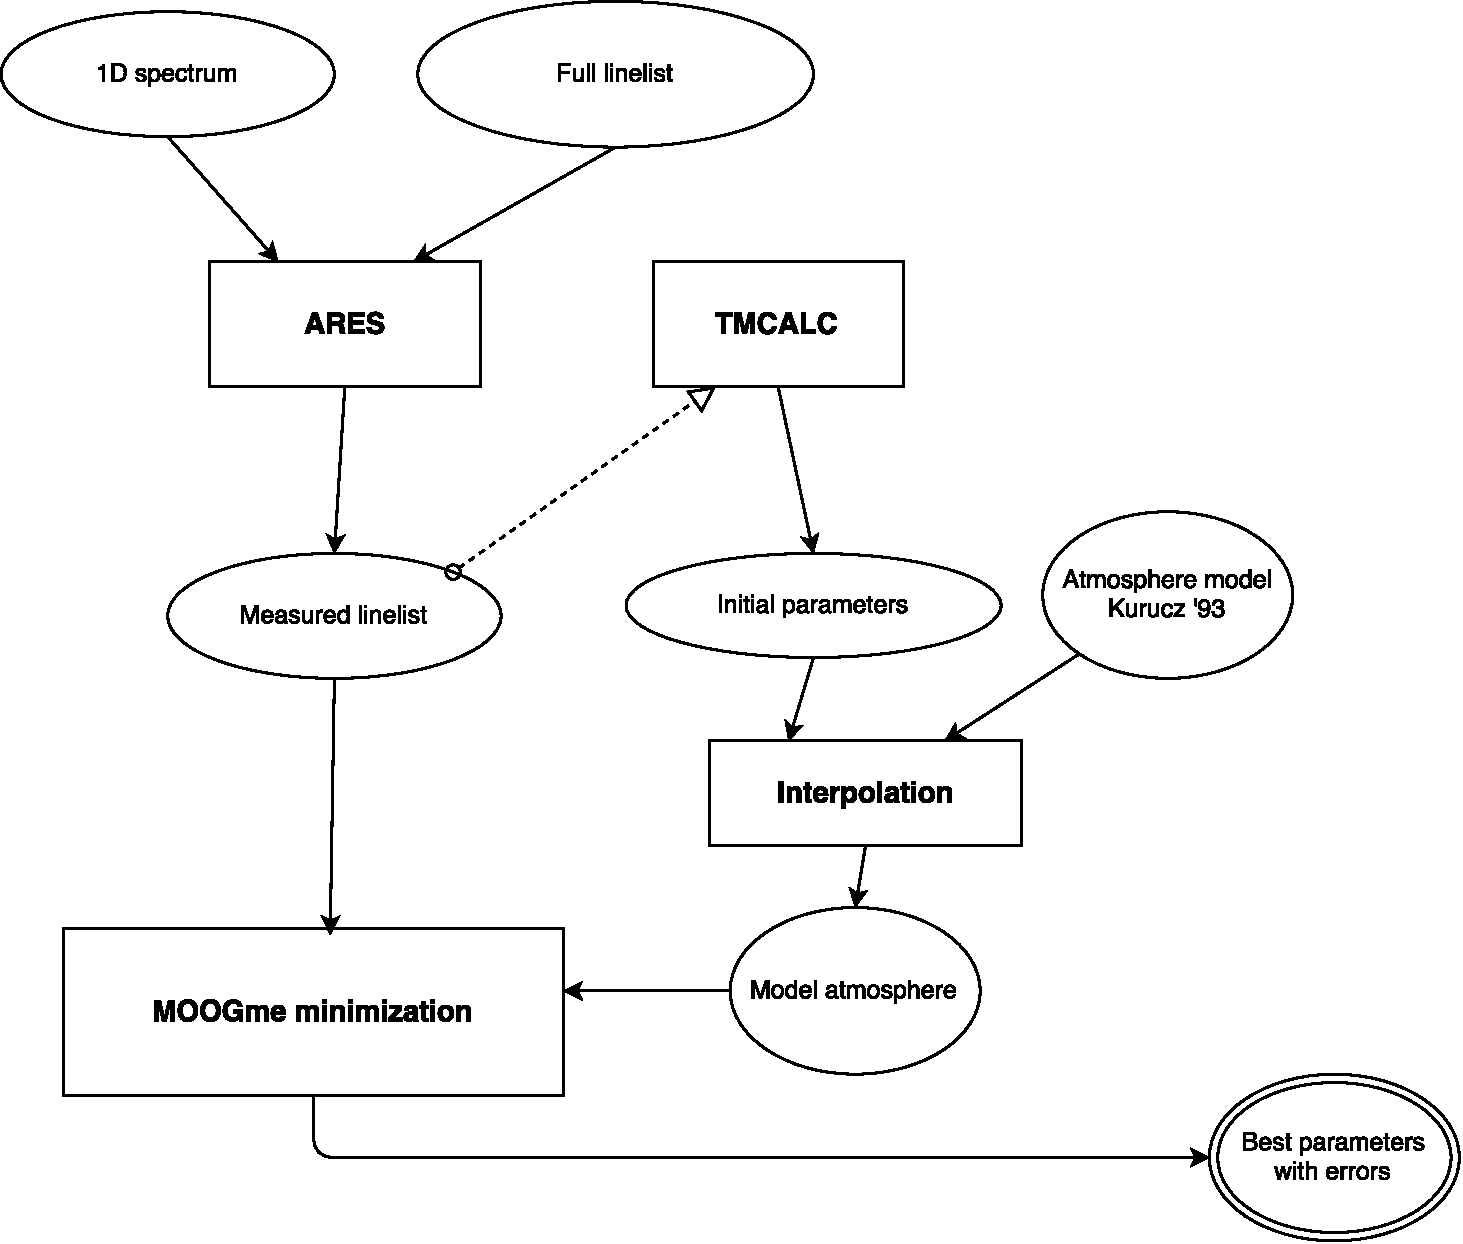
\includegraphics[width=1.0\linewidth]{figures/MOOGme_general.pdf}
    \caption{A general overview over MOOGme from spectrum to parameters.}
    \label{fig:MOOGme_general}
\end{figure}

There exists many minimization routines available in Python. Most commonly
known are the ones from the SciPy ecosystem\footnote{\url{http://scipy.org}}.
There are some pros and cons with using proprietary minimization routines.
Pros are that it is already written, and usually there are good documentation
in libraries such as SciPy. Cons in this situation is, that most minimization
routines are not able to handle multiple criteria at once. A work around is
to combine the criteria into one single criteria by e.g. adding them
quadratically and minimize that expression instead. The minimization routines
are also not physical in the sense that they are not optimized for the problem.
These two cons was incitement for writing a minimization optimized for our
problem. Here is how it works.

\begin{enumerate}
    \item Run MOOG once with a user defined initial parameters (default is
          solar) and calculate $a_\mathrm{EP}$, $a_\mathrm{RW}$, and
          $\Delta$\ion{Fe}.
    \item Change the atmospheric parameters ($T_\mathrm{eff}$, $\log g$,
          [\ion{Fe}/\ion{H}], $\xi_\mathrm{micro}$) according to the size of the
          indicator. A parameter is only changed if it is not fixed.
    \begin{itemize}
        \item $a_\mathrm{EP}$: Indicator for $T_\mathrm{eff}$. If this value
              is positive, then increase $T_\mathrm{eff}$.
        \item $a_\mathrm{RW}$: Same as above but for $\xi_\mathrm{micro}$.
        \item $\Delta$\ion{Fe}: Same as above but for $\log g$. Positive
              $\Delta$\ion{Fe} means $\log g$ should be decreased.
    \end{itemize}
    \item For [\ion{Fe}/\ion{H}] it is changed to the output [\ion{Fe}/\ion{H}]
          in each iteration (if free).
    \item If the new parameters have already been used in a previous, then
          change them slightly. This is done by drawing a random number from
          a Gaussian distribution with a mean at the previous value and a sigma
          equal to the absolute value of the indicator.
    \item Calculate a new atmospheric model by interpolating a grid so we have
          the requested parameters and run MOOG once again.
    \item For each iteration save the parameters used and the quadratic sum of
          the indicators. If we do not reach convergence, then return the best
          found parameters.
\end{enumerate}



\begin{figure}[tpb]
    \centering
    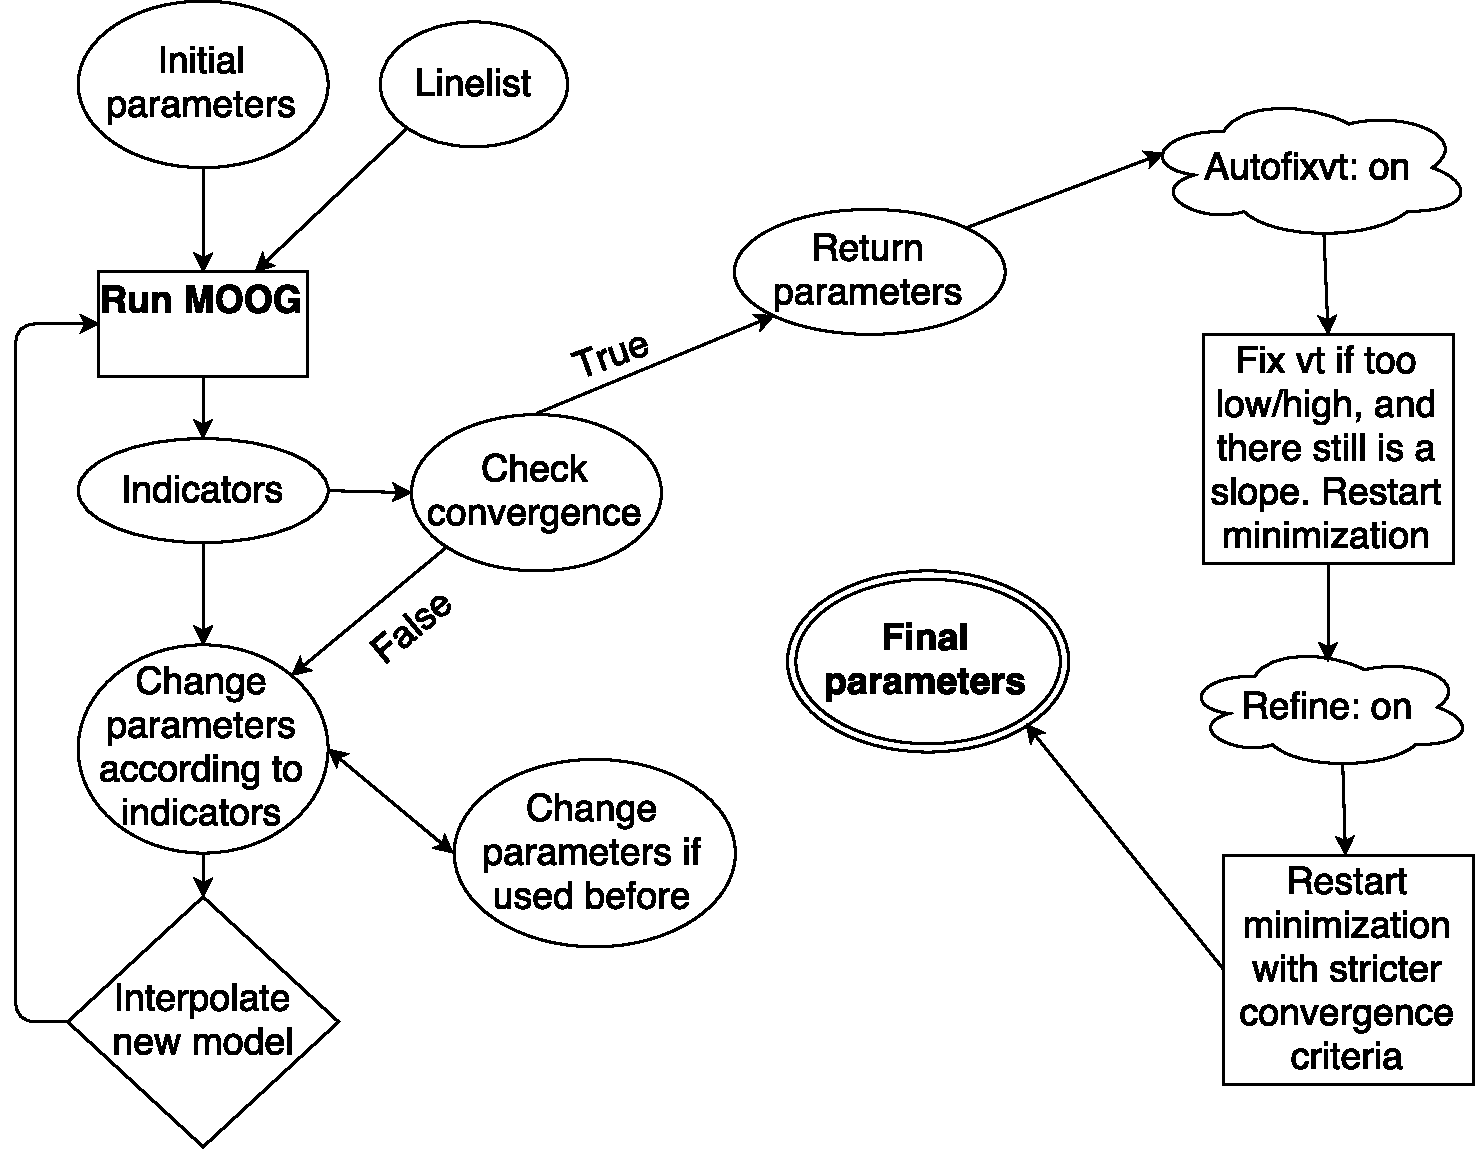
\includegraphics[width=1.0\linewidth]{figures/MOOGme_minimization.pdf}
    \caption{A schematic overview over the minimization for MOOGme with the
    EW method.}
    \label{fig:MOOGme_minimization}
\end{figure}




By using the indicators like this, we can relative fast reach convergence.
There are some interdependencies among the indicators. E.g. by changing
$T_\mathrm{eff}$ all indicators will be affected, however the effect is
strongest for $a_\mathrm{EP}$.

\subsubsection{Options}
\label{subs:EWoptions}
It is possible to run the EW method with a set of different options which
will be described here.

\begin{itemize}
    \item \emph{fixteff}: Fix $T_\mathrm{eff}$. Same is available for $\log g$
          (fixlogg), [\ion{Fe}/\ion{H}] (fixfeh), and $\xi_\mathrm{micro}$
          (fixvt).
    \item \emph{outlier}: Remove outliers after the first run with the minimization
          routine and restarting the minimization from the previous best
          parameters. The options are to remove all outliers above $3\sigma$
          once or iteratively, or remove one outlier above $3\sigma$ once or
          iteratively.
    \item \emph{autofixvt}: If the minimization routine does not converge and
          $\xi_\mathrm{micro}$ is close to 0 or 10 with a significant
          $a_\mathrm{RW}$, then fix $\xi_\mathrm{micro}$.
    \item \emph{refine}: After the minimization is done, run it again from the best
          found parameters but with more strict criteria. If this option is set,
          it will always be the last step (after removal of outliers and the
          use of teffrange).
\end{itemize}
If $\xi_\mathrm{micro}$ is fixed it is changed at each iteration according to
an empirical relation. For dwarfs it follows the one presented in
\citet{Tsantaki2013} and for giants it follows the one presented in
\citet{Adibekyan2015}. We use the line list presented in \citet{Sousa2008a}
for stars. However, this line list does not work well for cool stars. This
was fixed by \citet{Tsantaki2013} removing some lines from \citet{Sousa2008a}.
For stars cooler than \SI{5200}{K} we rederive the atmospheric parameters
after removing lines so the line list resemble that of \citet{Tsantaki2013}.

All restarts of the minimization routine is done with initial condition at
the last found best parameters.



\subsection{Abundance method}
\label{sub:Abundance_method}

We made a mode to calculate abundances for different elements based on the
measured EW. Here we require a line list with the EW of the elements and
the corresponding atmospheric parameters for the star of interest. We provide
a line list with XXX elements ready to use. The results are saved to a table.






\subsection{Testing MOOGme}
\label{sub:Testing_MOOGme}
To test the EW method implemented in MOOGme we derive
parameters from the 582 sample by \citet{Sousa2011}. We use ARES2
to measure the EWs. ARES can give an estimate on the signal to
noise ratio (SNR) by analyzing the continuum in given intervals.
For solar type stars the following intervals are working well:
\SIrange{5764}{5766}{\angstrom}, \SIrange{6047}{6053}{\angstrom}, and
\SIrange{6068}{6076}{\angstrom}. From the estimated SNR, ARES can give
an estimate on the very important \emph{rejt} parameters
\citep[see][for more information]{Sousa2015a}. After measuring the EWs
with ARES, we use the MOOGme minimization described in
Section~\ref{sub:EW_method} to determine the stellar atmospheric parameters.
The results are presented in Figure~\ref{fig:MOOGmeTest} which shows
$T_\mathrm{eff}$, $\log g$, [\ion{Fe}/\ion{H}], and $\xi_\mathrm{micro}$
for MOOGme against those of \citet{Sousa2011}.

\begin{figure*}[tpb]
    \centering
    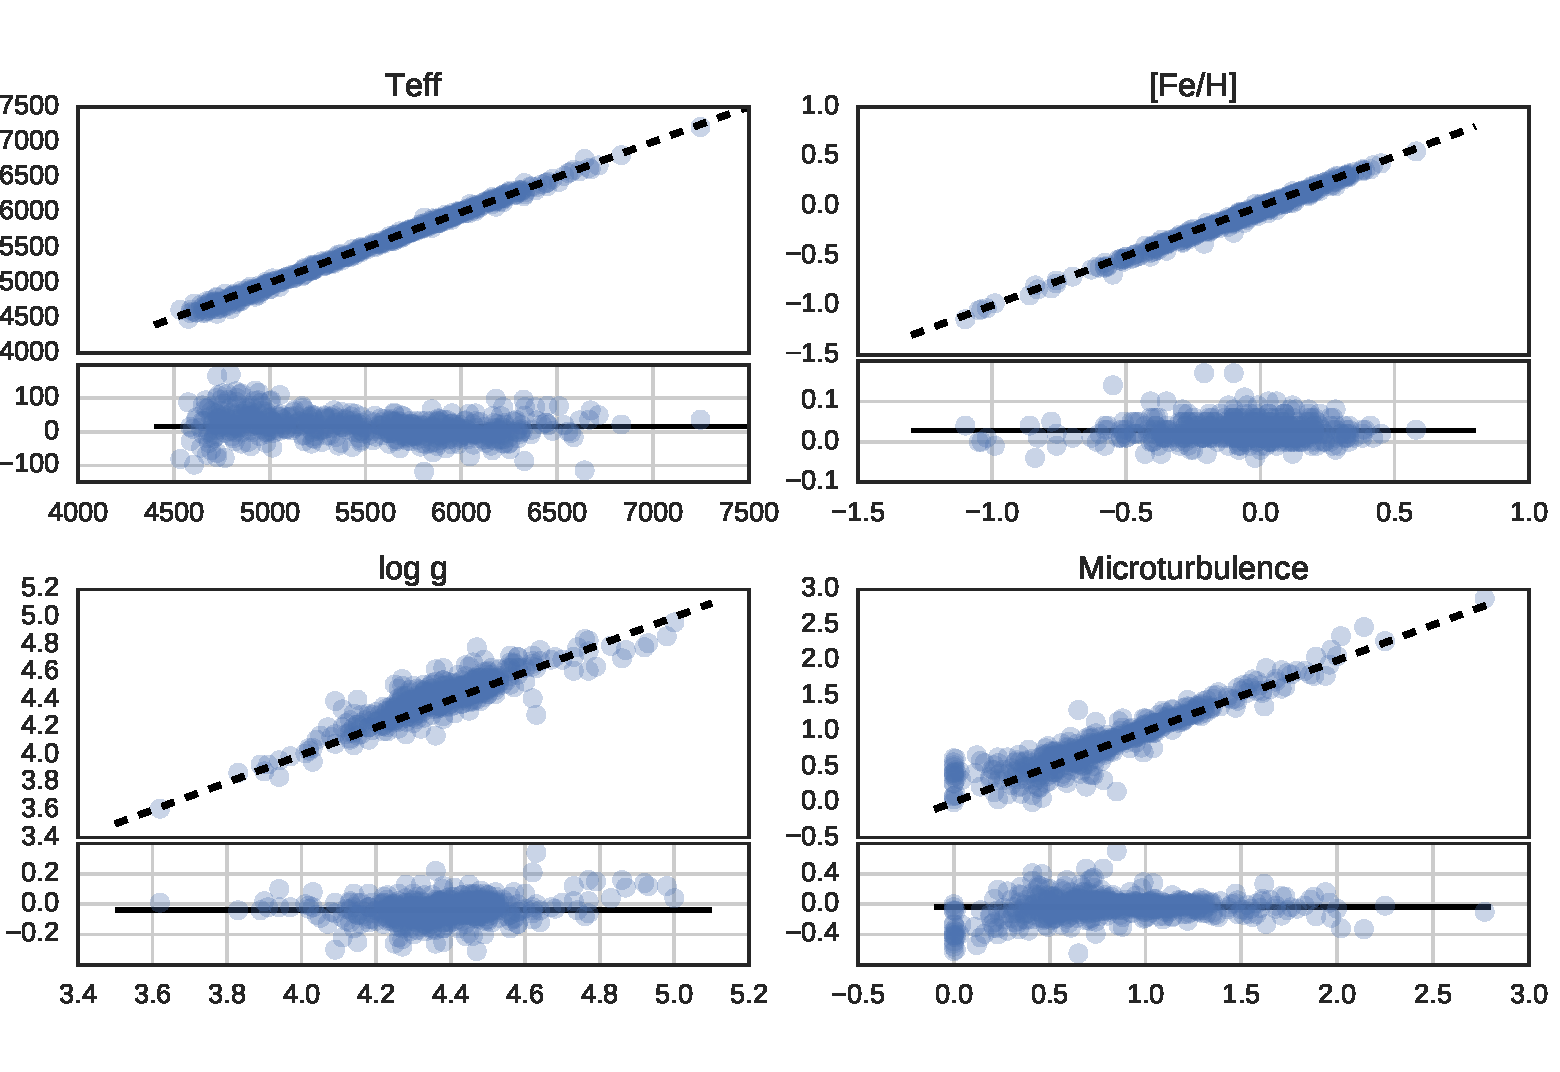
\includegraphics[width=1.0\linewidth]{figures/MOOGmeTest.pdf}
    \caption{Stellar atmospheric parameters derived by MOOGme compared
    to the sample by \citet{Sousa2011}.}
    \label{fig:MOOGmeTest}
\end{figure*}

The sample contains stars with $T_\mathrm{eff}$ too cold for the line
list used. As described in Section~\ref{sub:EW_method} we should then
apply the \emph{teffrange} option to compensate by converting the normal
line list by \citet{Sousa2008a} to the line list presented in \citet{Tsantaki2013}.
However, this line list was not available when \citet{Sousa2011} derived
parameters, hence we do not apply this option in order to make a better
test for MOOGme.

The mean of the difference between parameters from \citet{Sousa2011} and
those by MOOGme is presented in Table~\ref{tab:MOOGmeTest}.

\begin{table}[htb!]
    \caption{The difference in derived parameters by \citet{Sousa2011}
    and MOOGme.}
    \label{tab:MOOGmeTest}
    \centering
    \begin{tabular}{lrr}
      \hline\hline
      Parameter             &  Mean difference         & Mean difference (same line list) \\
      \hline
      $T_\mathrm{eff}$      &  $\SI{16(36)}{K}$        & $\SI{21(11)}{K}$                 \\
      $\log g$              &  $\num{-0.04(7)}$        & $\num{-0.007(9)}$                \\
      $[\ion{Fe}/\ion{H}]$  &  $\num{0.03(2)}$         & $\num{0.004(9)}$                 \\
      $\xi_\mathrm{micro}$  &  $\SI{-0.04(14)}{km/s}$  & $\SI{0.04(2)}{km/s}$             \\
      \hline
    \end{tabular}
\end{table}

We see small offsets that can be due to different versions of MOOG, different
line lists, and different minimization routine. We therefore randomly
selected 20 stars with different $T_\mathrm{eff}$ and used the line list
directly from \citet{Sousa2011} to derive parameters. The results are
presented in the last column of Table~\ref{tab:MOOGmeTest}. We note that
the $\log gf$ values from the original line lists by \citet{Sousa2011}, which
used the MOOG 2002 version, were not changed for the 2014 version of MOOG.
This might lead to some errors as well. However, the offsets are very small
and compatible with the errors on parameters normally obtained from high
quality spectra.


\subsection{Web interface}
\label{sub:Web interface}
We provide a web interface for MOOGme. In the web interface it is
possible to use some of the line list provided with MOOGme to
measure EWs of a spectrum (has to be provided by the user). This
can be used for all the available MOOGme methods described above.

The web interface can be found at the following link
\url{super-cool-address-with-MOOGme}.



\section{New spectroscopic parameters for 49 planet hosts}
\label{sec:results}
Here we present the sample of 50 stars. We were unable to derive parameters for
HD77065. This is a spectroscopic binary according to \cite{Pourbaix2004}.

The remaining 49 stars are presented in Table~\ref{tab:results}.


\begin{table*}[htb!]
    \caption{The derived parameters for the 49 stars in our sample.}
    \label{tab:results}
    \centering
    \begin{tabular}{lllllll}
      \hline\hline
      % Add alternative name and SNR
        Star      & $T_\mathrm{eff}$ (K) &  $\log g$ (dex)     &  [Fe/H] (dex)        &  $\xi_\mathrm{micro}$ (km/s) & $\xi_\mathrm{micro}$ fixed? & Program ID \\
      \hline
      WASP-76     &  $6347 \pm  52$      &  $4.29 \pm 0.08$    &  $ 0.36 \pm 0.04$    &  $1.73 \pm 0.06$             &             no              &  2014B/020,  094.C-0367                                                                                                  \\
      WASP-82     &  $6563 \pm  55$      &  $4.29 \pm 0.10$    &  $ 0.18 \pm 0.04$    &  $1.93 \pm 0.08$             &             no              &  2014B/020,  094.C-0367                                                                                                  \\
      WASP-88     &  $6450 \pm  61$      &  $4.24 \pm 0.06$    &  $ 0.03 \pm 0.04$    &  $1.79 \pm 0.09$             &             no              &  2014B/020,  095.C-0324                                                                                                  \\
      WASP-95     &  $5799 \pm  31$      &  $4.29 \pm 0.05$    &  $ 0.22 \pm 0.03$    &  $1.18 \pm 0.04$             &             no              &  2014B/020,  095.C-0324                                                                                                  \\
      WASP-97     &  $5723 \pm  52$      &  $4.37 \pm 0.07$    &  $ 0.31 \pm 0.04$    &  $1.03 \pm 0.08$             &             no              &  2014B/020,  094.C-0367                                                                                                  \\
      WASP-99     &  $6324 \pm  89$      &  $4.70 \pm 0.11$    &  $ 0.27 \pm 0.06$    &  $1.83 \pm 0.12$             &             no              &  2014B/020,  094.C-0367                                                                                                  \\
       HATS-1     &  $5969 \pm  46$      &  $4.61 \pm 0.06$    &  $-0.04 \pm 0.04$    &  $1.06 \pm 0.08$             &             no              &  092.C-0695                                                                                                              \\
      Qatar-2     &  $4637 \pm 316$      &  $4.23 \pm 0.61$    &  $ 0.09 \pm 0.17$    &  $0.63 \pm 0.83$             &             no              &  092.C-0695                                                                                                              \\
      WASP-44     &  $5612 \pm  80$      &  $4.47 \pm 0.30$    &  $ 0.17 \pm 0.06$    &  $1.32 \pm 0.13$             &             no              &  092.C-0695                                                                                                              \\
     HAT-P-46     &  $6421 \pm 121$      &  $4.53 \pm 0.14$    &  $ 0.16 \pm 0.09$    &  $1.67 \pm 0.18$             &             no              &  093.C-0219                                                                                                              \\
      WASP-52     &  $5197 \pm  83$      &  $4.47 \pm 0.30$    &  $ 0.15 \pm 0.05$    &  $1.16 \pm 0.14$             &             no              &  093.C-0219                                                                                                              \\
      WASP-72     &  $6570 \pm  85$      &  $4.71 \pm 0.13$    &  $ 0.15 \pm 0.06$    &  $2.30 \pm 0.15$             &             no              &  093.C-0219                                                                                                              \\
      WASP-75     &  $6203 \pm  46$      &  $4.42 \pm 0.22$    &  $ 0.24 \pm 0.03$    &  $1.45 \pm 0.06$             &             no              &  093.C-0219                                                                                                              \\
     HAT-P-42     &  $5903 \pm  66$      &  $4.29 \pm 0.10$    &  $ 0.34 \pm 0.05$    &  $1.19 \pm 0.08$             &             no              &  094.C-0367                                                                                                              \\
       HATS-5     &  $5383 \pm  91$      &  $4.40 \pm 0.22$    &  $ 0.08 \pm 0.06$    &  $0.91 \pm 0.14$             &             no              &  094.C-0367                                                                                                              \\
    HD 285507     &  $4620 \pm 126$      &  $4.42 \pm 0.61$    &  $ 0.04 \pm 0.06$    &  $0.74 \pm 0.43$             &             no              &  094.C-0367                                                                                                              \\
       HR 228     &  $5042 \pm  42$      &  $3.30 \pm 0.09$    &  $ 0.07 \pm 0.03$    &  $1.14 \pm 0.04$             &             no              &  094.C-0367                                                                                                              \\
      SAND364     &  $4457 \pm 104$      &  $2.26 \pm 0.20$    &  $-0.04 \pm 0.06$    &  $1.60 \pm 0.11$             &             no              &  094.C-0367                                                                                                              \\
       GJ 785     &  $5087 \pm  48$      &  $4.30 \pm 0.10$    &  $-0.01 \pm 0.03$    &  $0.69 \pm 0.10$             &             no              &  60.A-9036(A), 072.C-0488(E), 081.C-0842(D), 083.C-1001(A)                                                               \\
    HD 120084     &  $4969 \pm  40$      &  $2.94 \pm 0.14$    &  $ 0.12 \pm 0.03$    &  $1.41 \pm 0.04$             &             no              &  14AF14                                                                                                                  \\
    HD 192263     &  $4946 \pm  46$      &  $4.43 \pm 0.14$    &  $-0.05 \pm 0.02$    &  $0.66 \pm 0.12$             &             no              &  087.C-0012(B), 192.C-0852(A)                                                                                            \\
   HIP 107773     &  $4957 \pm  49$      &  $2.83 \pm 0.09$    &  $ 0.04 \pm 0.04$    &  $1.49 \pm 0.05$             &             no              &  085.C-0062(A)                                                                                                           \\
    HD 219134     &  $4767 \pm  70$      &  $4.32 \pm 0.17$    &  $-0.00 \pm 0.04$    &  $0.59 \pm 0.24$             &             no              &  07bo03                                                                                                                  \\
     HD 81688     &  $4906 \pm  29$      &  $2.69 \pm 0.06$    &  $-0.21 \pm 0.02$    &  $1.60 \pm 0.03$             &             no              &  14AF14, 53-202                                                                                                          \\
     HD 82886     &  $5124 \pm  22$      &  $3.30 \pm 0.05$    &  $-0.25 \pm 0.02$    &  $1.15 \pm 0.03$             &             no              &  14AF14, 53-202                                                                                                          \\
       mu Leo     &  $4605 \pm  94$      &  $2.61 \pm 0.26$    &  $ 0.25 \pm 0.06$    &  $1.64 \pm 0.11$             &             no              &  11AQ78, 05AC23, 06AF22                                                                                                  \\
     HD 87883     &  $4917 \pm  68$      &  $4.34 \pm 0.19$    &  $ 0.02 \pm 0.03$    &  $0.46 \pm 0.21$             &             no              &  14AF14                                                                                                                  \\
    HIP 11915     &  $5770 \pm  14$      &  $4.47 \pm 0.03$    &  $-0.06 \pm 0.01$    &  $0.95 \pm 0.02$             &             no              &  072.C-0488(E), 089.C-0732(A), 091.C-0034(A), 092.C-0721(A), 093.C-0409(A), 183.C-0972(A), 188.C-0265(A), 192.C-0852(M)  \\
      omi UMa     &  $5499 \pm  52$      &  $3.36 \pm 0.07$    &  $-0.01 \pm 0.05$    &  $1.98 \pm 0.06$             &             no              &  14AF14                                                                                                                  \\
       11 Com     &  $4911 \pm  38$      &  $2.68 \pm 0.08$    &  $-0.20 \pm 0.03$    &  $1.56 \pm 0.04$             &             no              &  53-202                                                                                                                  \\
    HD 102272     &  $5037 \pm  80$      &  $2.72 \pm 0.25$    &  $-0.52 \pm 0.08$    &  $0.67 \pm 0.12$             &             no              &  53-202                                                                                                                  \\
    HD 104985     &  $4809 \pm  48$      &  $2.73 \pm 0.08$    &  $-0.26 \pm 0.04$    &  $1.65 \pm 0.05$             &             no              &  53-202                                                                                                                  \\
    HD 114762     &  $6061 \pm  83$      &  $4.70 \pm 0.08$    &  $-0.78 \pm 0.05$    &  $0.02 \pm 0.26$             &             no              &  53-202                                                                                                                  \\
      omi CrB     &  $4915 \pm  33$      &  $2.74 \pm 0.08$    &  $-0.14 \pm 0.03$    &  $1.57 \pm 0.04$             &             no              &  53-202                                                                                                                  \\
    HD 152581     &  $5355 \pm  82$      &  $3.65 \pm 0.18$    &  $-0.39 \pm 0.07$    &  $0.60 \pm 0.15$             &             no              &  095.C-0324, 53-202                                                                                                      \\
    HD 155358     &  $5917 \pm  51$      &  $4.12 \pm 0.08$    &  $-0.55 \pm 0.04$    &  $1.06 \pm 0.08$             &             no              &  40-203                                                                                                                  \\
       42 Dra     &  $4547 \pm  55$      &  $2.23 \pm 0.10$    &  $-0.31 \pm 0.03$    &  $1.54 \pm 0.05$             &             no              &  49-202                                                                                                                  \\
    HD 220842     &  $6027 \pm  30$      &  $4.35 \pm 0.05$    &  $-0.08 \pm 0.03$    &  $1.19 \pm 0.04$             &             no              &  44-210                                                                                                                  \\
       14 And     &  $4797 \pm  44$      &  $2.58 \pm 0.11$    &  $-0.23 \pm 0.03$    &  $1.58 \pm 0.04$             &             no              &  49-202                                                                                                                  \\
    HD 233604     &  $4925 \pm  44$      &  $2.79 \pm 0.11$    &  $-0.15 \pm 0.03$    &  $1.62 \pm 0.05$             &             no              &  53-202                                                                                                                  \\
     HD 37124     &  $5468 \pm  32$      &  $4.28 \pm 0.04$    &  $-0.43 \pm 0.03$    &  $0.67 \pm 0.07$             &             no              &  53-202                                                                                                                  \\
     HD 97658     &  $5182 \pm  43$      &  $4.50 \pm 0.12$    &  $-0.29 \pm 0.03$    &  $0.77 \pm 0.11$             &             no              &  53-202                                                                                                                  \\
   Kepler-444     &  $5163 \pm  40$      &  $4.41 \pm 0.11$    &  $-0.50 \pm 0.03$    &  $0.78 \pm 0.10$             &             no              &  53-202                                                                                                                  \\
     WASP-100     &  $6853 \pm 209$      &  $4.15 \pm 0.26$    &  $-0.30 \pm 0.12$    &  $1.87 \pm 0.02$             &             yes             &  2014B/020  094.C-0367                                                                                                   \\
     HAT-P-24     &  $6470 \pm 181$      &  $4.75 \pm 0.26$    &  $-0.41 \pm 0.10$    &  $1.40 \pm 0.03$             &             yes             &  092.C-0695                                                                                                              \\
     HAT-P-39     &  $6745 \pm 236$      &  $4.91 \pm 0.46$    &  $-0.21 \pm 0.12$    &  $1.53 \pm 0.04$             &             yes             &  094.C-0367                                                                                                              \\
      WASP-61     &  $6265 \pm 168$      &  $4.21 \pm 0.21$    &  $-0.38 \pm 0.11$    &  $1.44 \pm 0.02$             &             yes             &  094.C-0367                                                                                                              \\
     HD 70573     &  $5889 \pm 186$      &  $4.32 \pm 0.27$    &  $-0.42 \pm 0.13$    &  $1.14 \pm 0.01$             &             yes             &  53-202                                                                                                                  \\
      \hline
    \end{tabular}
\end{table*}


We present a Hertzprung-Russel diagram (HRD) of our sample in
Figure~\ref{fig:HRD}.
\begin{figure}[tpb]
    \centering
    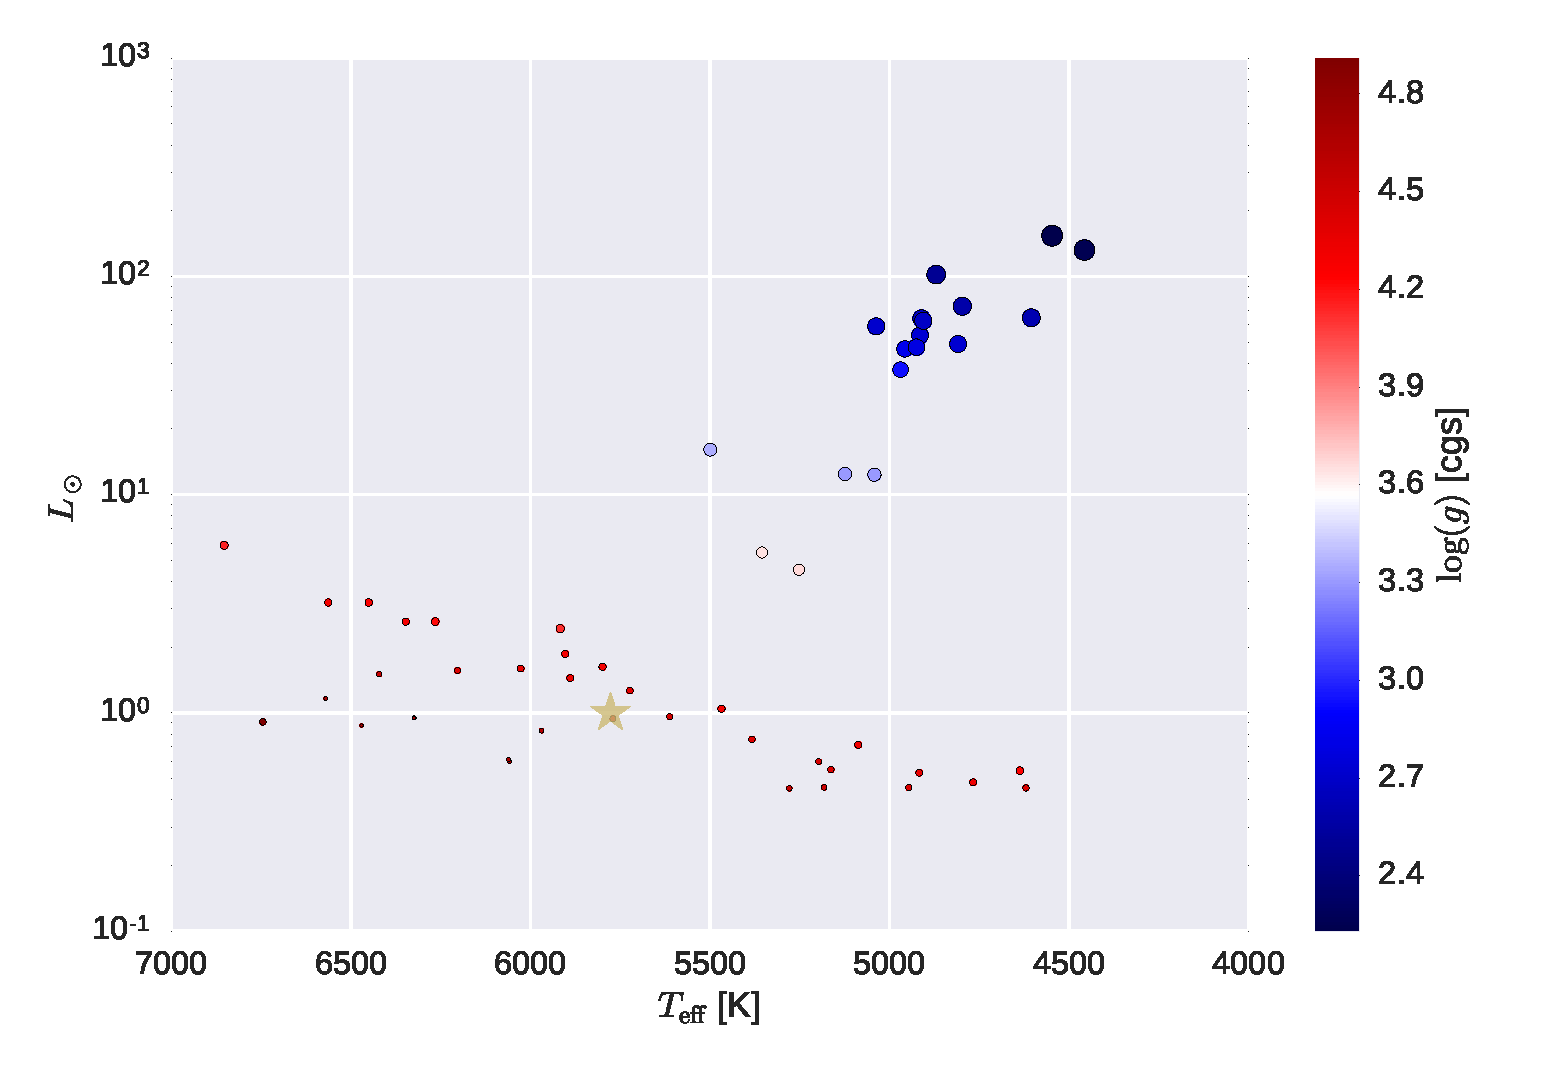
\includegraphics[width=1.0\linewidth]{figures/HR.pdf}
    \caption{Hertzprung-Russel diagram of our sample with the Sun as a yellow
    star. The size of the points represents the $\log g$, with bigger points
    being smaller $\log g$ (giants), and vice versa. The colour code show the
    same as the size. Red points are the dwarfs, while blue points are the
    giants.}
    \label{fig:HRD}
\end{figure}

Figure~\ref{fig:HRD} is made with a tool for post processing the results
saved to a table by MOOGme. We also use \emph{isochrones} \citep{Morton2015}
to give an estimate of the age. The mass estimation is based on the relation
by \citet{Torres2010}. The age estimation is dependent on the mass of the
star and the metallicity, which can be seen Figure~\ref{fig:age}.

\begin{figure}[tpb]
    \centering
    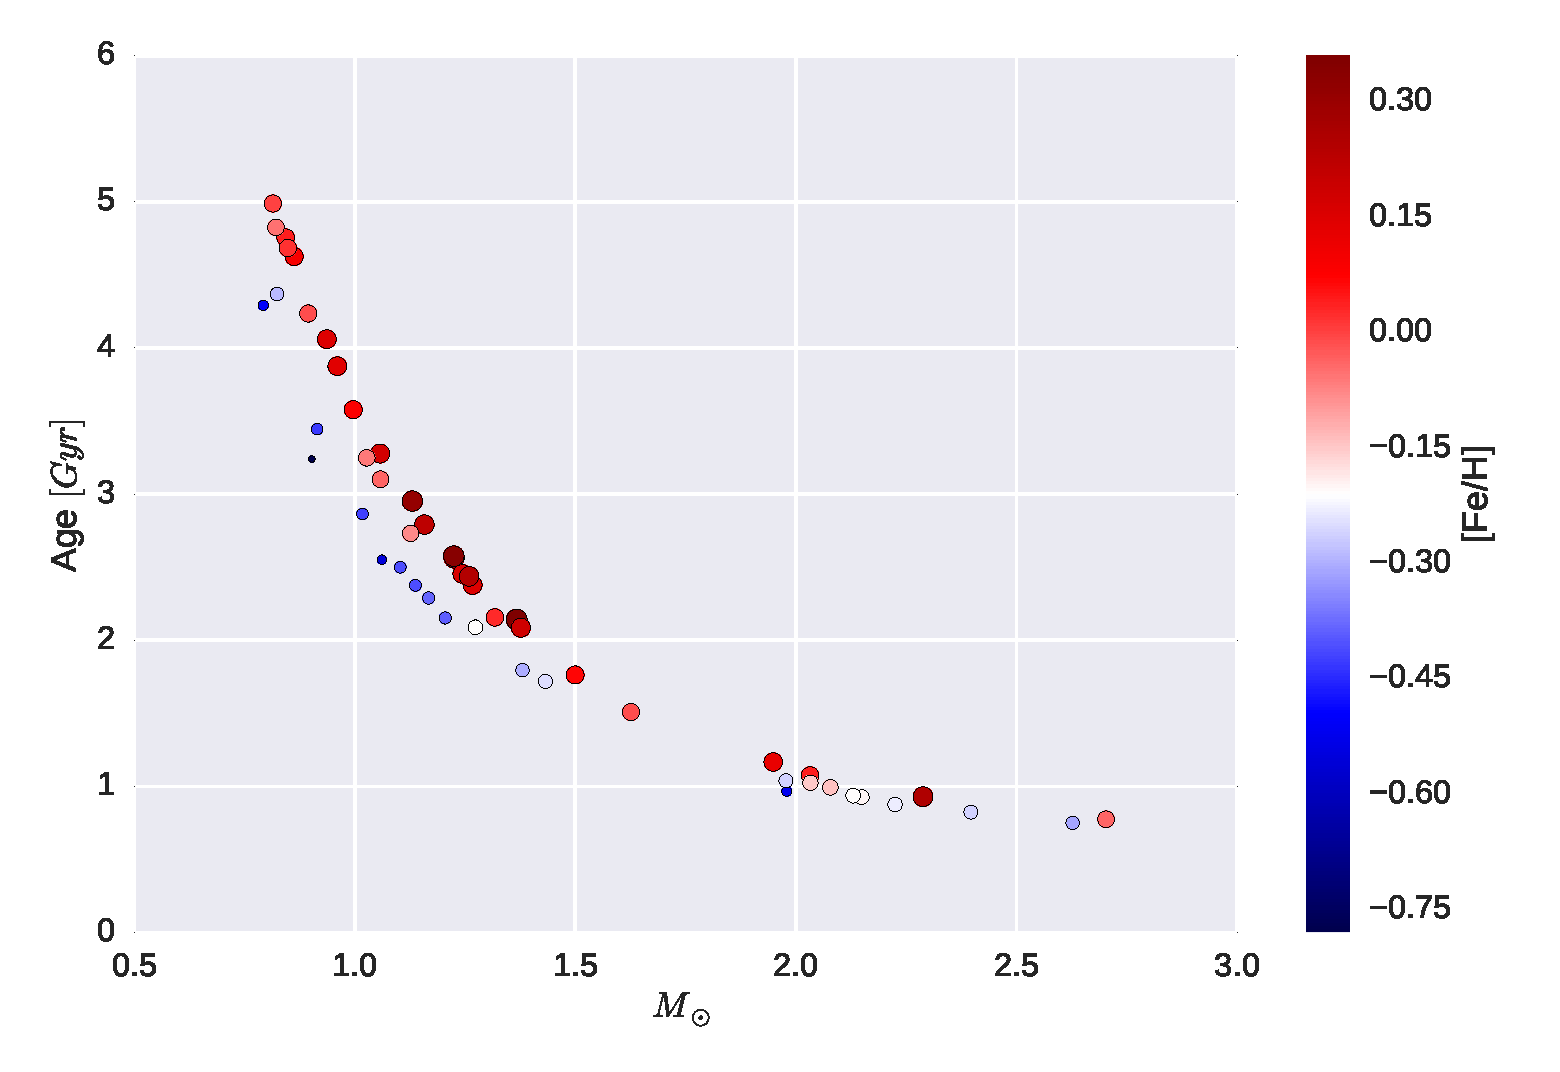
\includegraphics[width=1.0\linewidth]{figures/mass_age_feh.pdf}
    \caption{Age versus mass for our sample, with colours representing the
    [\ion{Fe}/\ion{H}].}
    \label{fig:age}
\end{figure}



\section{Conclusion}
\label{sec:conclusion}




\begin{acknowledgements}

This work was supported by Funda\c{c}\~ao para a Ci\^encia e a
Tecnologia (FCT) through the research grants UID/FIS/04434/2013 and
PTDC/FIS-AST/1526/2014. N.C.S., and S.G.S. acknowledge the support from
FCT through Investigador FCT contracts of reference IF/00169/2012, and
IF/00028/2014, respectively, and POPH/FSE (EC) by FEDER funding through
the program “Programa Operacional de Factores de Competitividade
- COMPETE”. E.D.M. and B.J.A. acknowledge the support from FCT in
form of the fellowship SFRH/BPD/76606/2011 and SFRH/BPD/87776/2012,
respectively. This work also benefit from the collaboration of a
cooperation project FCT/CAPES - 2014/2015 (FCT Proc 4.4.1.00 CAPES).

AM received funding from the European Union Seventh Framework Programme
(FP7/2007-2013) under grant agreement number 313014 (ETAEARTH).


This research has made use of the SIMBAD database operated at CDS,
Strasbourg (France).

\end{acknowledgements}


\bibpunct{(}{)}{;}{a}{}{,}
\bibliographystyle{aa}
\bibliography{thesis}



\end{document}
